\documentclass[9pt, aspectratio=169]{beamer}
\usepackage{FiraSans}
\usetheme[subsectionpage=progressbar]{metropolis}
\usepackage[utf8]{inputenc}
\usepackage{amsmath}
\usepackage{amsfonts}
\usepackage{amssymb}
\usepackage{multicol}
\usepackage{tikz}
\usetikzlibrary{decorations.pathreplacing}
\usetikzlibrary{fadings}
\usepackage{caption}
\usepackage{xcolor}
\usepackage[T1]{fontenc} 
\usepackage[skins]{tcolorbox}
\author{Nicola Roman\`o - nicola.romano@ed.ac.uk}
\title{Lecture 10 - Introduction to neural networks}
\setlength{\fboxsep}{0pt}
\setbeamertemplate {footline}{\begin{scriptsize}\hfill\insertframenumber ~of \inserttotalframenumber\kern1em\vskip5pt\end{scriptsize}}

% Remove "Figure" in front of captions
% See https://tex.stackexchange.com/questions/82456/how-to-remove-figure-caption-prefix-figure-in-beamer
\captionsetup{labelformat=empty,labelsep=none}

\titlegraphic{\centering 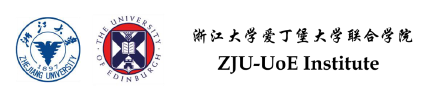
\includegraphics[scale=.5]{instituteLogo.png}}
\date{}

\begin{document}

\newtcolorbox{codebox}{enhanced,
    top=2pt,
    left=2pt,
    right=2pt,
    bottom=2pt,
    boxrule=0pt,
    leftrule=5pt,
    sharp corners,
    colback=gray!20,
    colframe=blue!60!black}

\begin{frame}
    \titlepage
\end{frame}

\begin{frame}
    {Learning objectives}
    \begin{columns}
        \begin{column}{0.8\textwidth}
            \begin{itemize}
                \item Describe artificial neural networks (ANNs).
                \item Explain the learning process of ANNs.
                \item Explain the concept of gradient descent.
            \end{itemize}
        \end{column}
        \begin{column}{0.2\textwidth}
            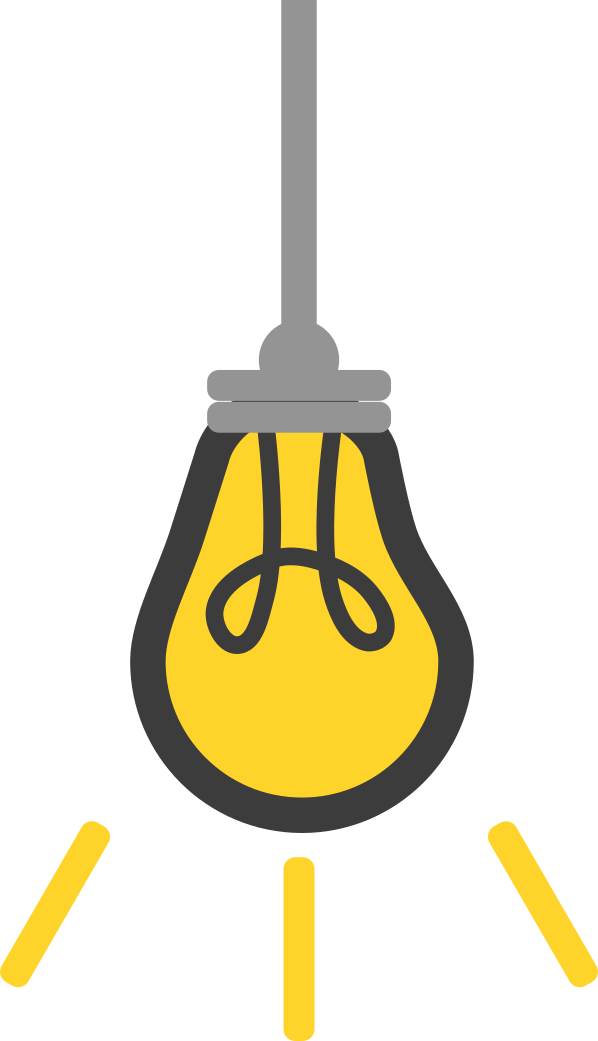
\includegraphics[angle=-30, origin=tr, width=1.5\textwidth]{lightbulb.png}
        \end{column}
    \end{columns}
\end{frame}

\section{Introduction}

\begin{frame}
    {Artificial neural networks}
    An artificial neural network (ANN) is a supervised computing algorithm made up of nodes (\textbf{neurons}) that loosely resemble biological neurons.

    \pause

    Each neuron takes in a number of inputs, performs some calculation on these inputs and outputs anothe value.

    The connections between neurons (\textbf{edges}) are weighted, so that different inputs might influence the results in different ways.

    Typically, neural networks consists of layers of these nodes.
\end{frame}

\begin{frame}
    {Why using neural networks?}

    \begin{itemize}
        \item Used in many field - adaptable to many problems
        \item Sufficiently complex networks can approximate any function
        \item Image analysis / computer vision has vastly benefitted from ANN (specifically CNN) as they can extract complex information from images
        \item Downside: often network computation is difficult to interpret
    \end{itemize}
    \pause

    Today we will introduce \textbf{shallow networks}, and will move onto \textbf{deep networks} in the next lectures.
\end{frame}

\section{Single layer ANN}

\begin{frame}
    {The McCulloch-Pitts Neuron}

    \begin{itemize}
        \item Linear threshold unit (LTU)
        \item The first type of artificial neuron developed in 1943 by McCulloch and Pitts
        \item Little resemblance to biological neurons
        \item Only very simple (binary) operation possible
        \item Inputs can only be 0 or 1, weights could be +1 or -1 (excitatory or inhibitory)
        \item A simple \textbf{threshold} $T$ decides the binary output.
    \end{itemize}

    \centering
    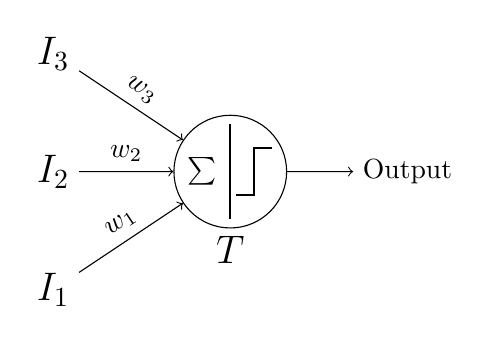
\begin{tikzpicture}[scale=1.5]
        % Neuron
        \node [draw, fill=white, circle, minimum height=4em] (n) at(1.5, 1) {$\sum\qquad$};
        \node [below of = n] {\Large\textbf{$T$}};

        % Inputs and weights
        \foreach \i in {1,2,3}
            {
                \node (i\i) at(0,\i-1) {\Large$I_\i$};
                \draw [->] (i\i) -- node [above, midway, sloped] {\textbf{$w_\i$}} (n);
            }

        \node (out) at(3, 1) {Output};
        \draw [->] (n) -- (out);
        \draw [thick] (1.5, .6) -- (1.5, 1.4);

        \draw [thick] (1.55, 0.8) -- (1.7, 0.8) -- (1.7, 1.2) -- (1.85, 1.2);

    \end{tikzpicture}
\end{frame}

\begin{frame}
    {The perceptron}
    \begin{columns}
        \begin{column}{.5\textwidth}
            \begin{itemize}
                \item A much more useful/powerful ANN
                \item Developed by Frank Rosenblatt in 1945
                \item Used as a binary classifier
                      \pause
                \item Learns:\qquad $f(\mathbf{x}) = \begin{cases}1 & \text{if }\ \mathbf{w} \cdot \mathbf{x} + b > 0,\\0 & \text{otherwise}\end{cases}$\\
                      $\mathbf{x}$: vector of input features\\
                      $\mathbf{w}$: vector of weights\\
                      $b$: bias
            \end{itemize}
        \end{column}
        \begin{column}{.5\textwidth}
            \only<3>{
                \begin{itemize}
                    \item Includes an \textbf{activation function} (e.g. a sigmoid), which can introduce non-linearity in the system, allowing to model complex functions.
                    \item Includes a \textbf{bias term}, which allows shifting the activation function.
                \end{itemize}
            }
        \end{column}
    \end{columns}

    \centering
    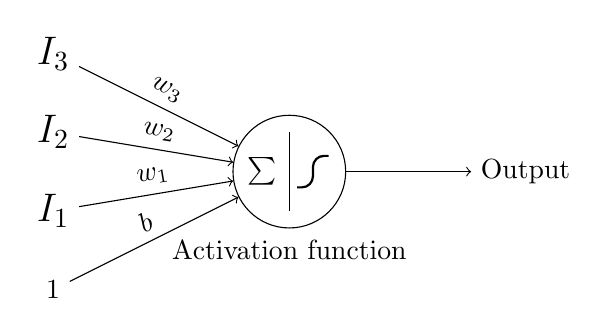
\begin{tikzpicture}
        % Neuron
        \node [draw, fill=white, circle, minimum height=4em] (n) at(3, 1.5) {$\sum\qquad$};

        \node [below of = n] {Activation function};

        % Bias
        \node (b) at(0, 0) {1};
        \draw [->] (b) -- node [above, midway, sloped] {\textbf{$b$}} (n);

        % Inputs and weights
        \foreach \i in {1,2,3}
            {
                \node (i\i) at(0,\i) {\Large$I_\i$};
                \draw [->] (i\i) -- node [above, midway, sloped] {\textbf{$w_\i$}} (n);
            }

        \node (out) at(6, 1.5) {Output};
        \draw [->] (n) -- (out);

        \draw [thick, rounded corners] (3.1, 1.3) -- (3.3, 1.3) -- (3.3, 1.7) -- (3.5, 1.7);

        \draw (3, 1) -- (3, 2);
    \end{tikzpicture}
\end{frame}

\begin{frame}
    {A little historical side note...}
    The perceptron was built as an actual machine!

    \begin{columns}
        \begin{column}{.5\textwidth}
            \centering
            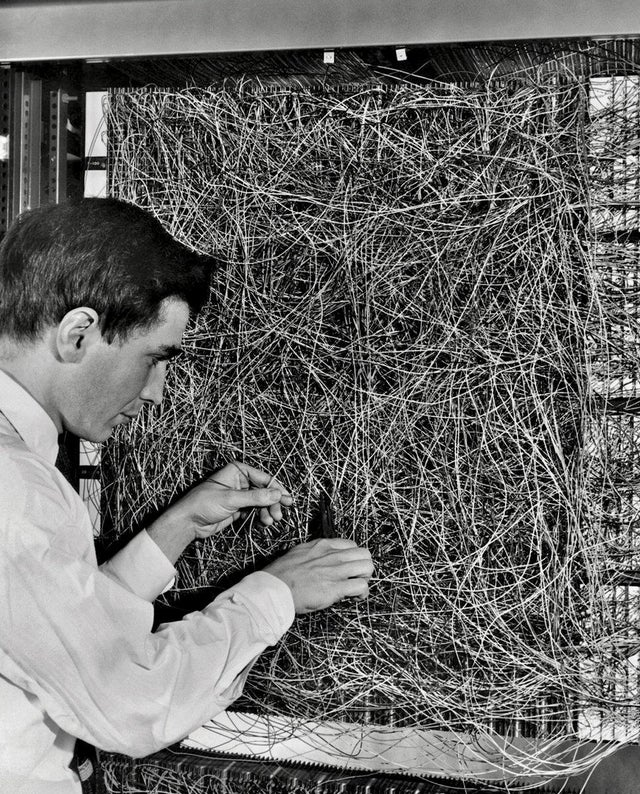
\includegraphics[height=.7\textheight]{MarkI_perceptron.jpg}

            \footnotesize
            Frank Rosenblatt with a Mark I Perceptron computer in 1960
        \end{column}
        \begin{column}{.5\textwidth}
            \centering
            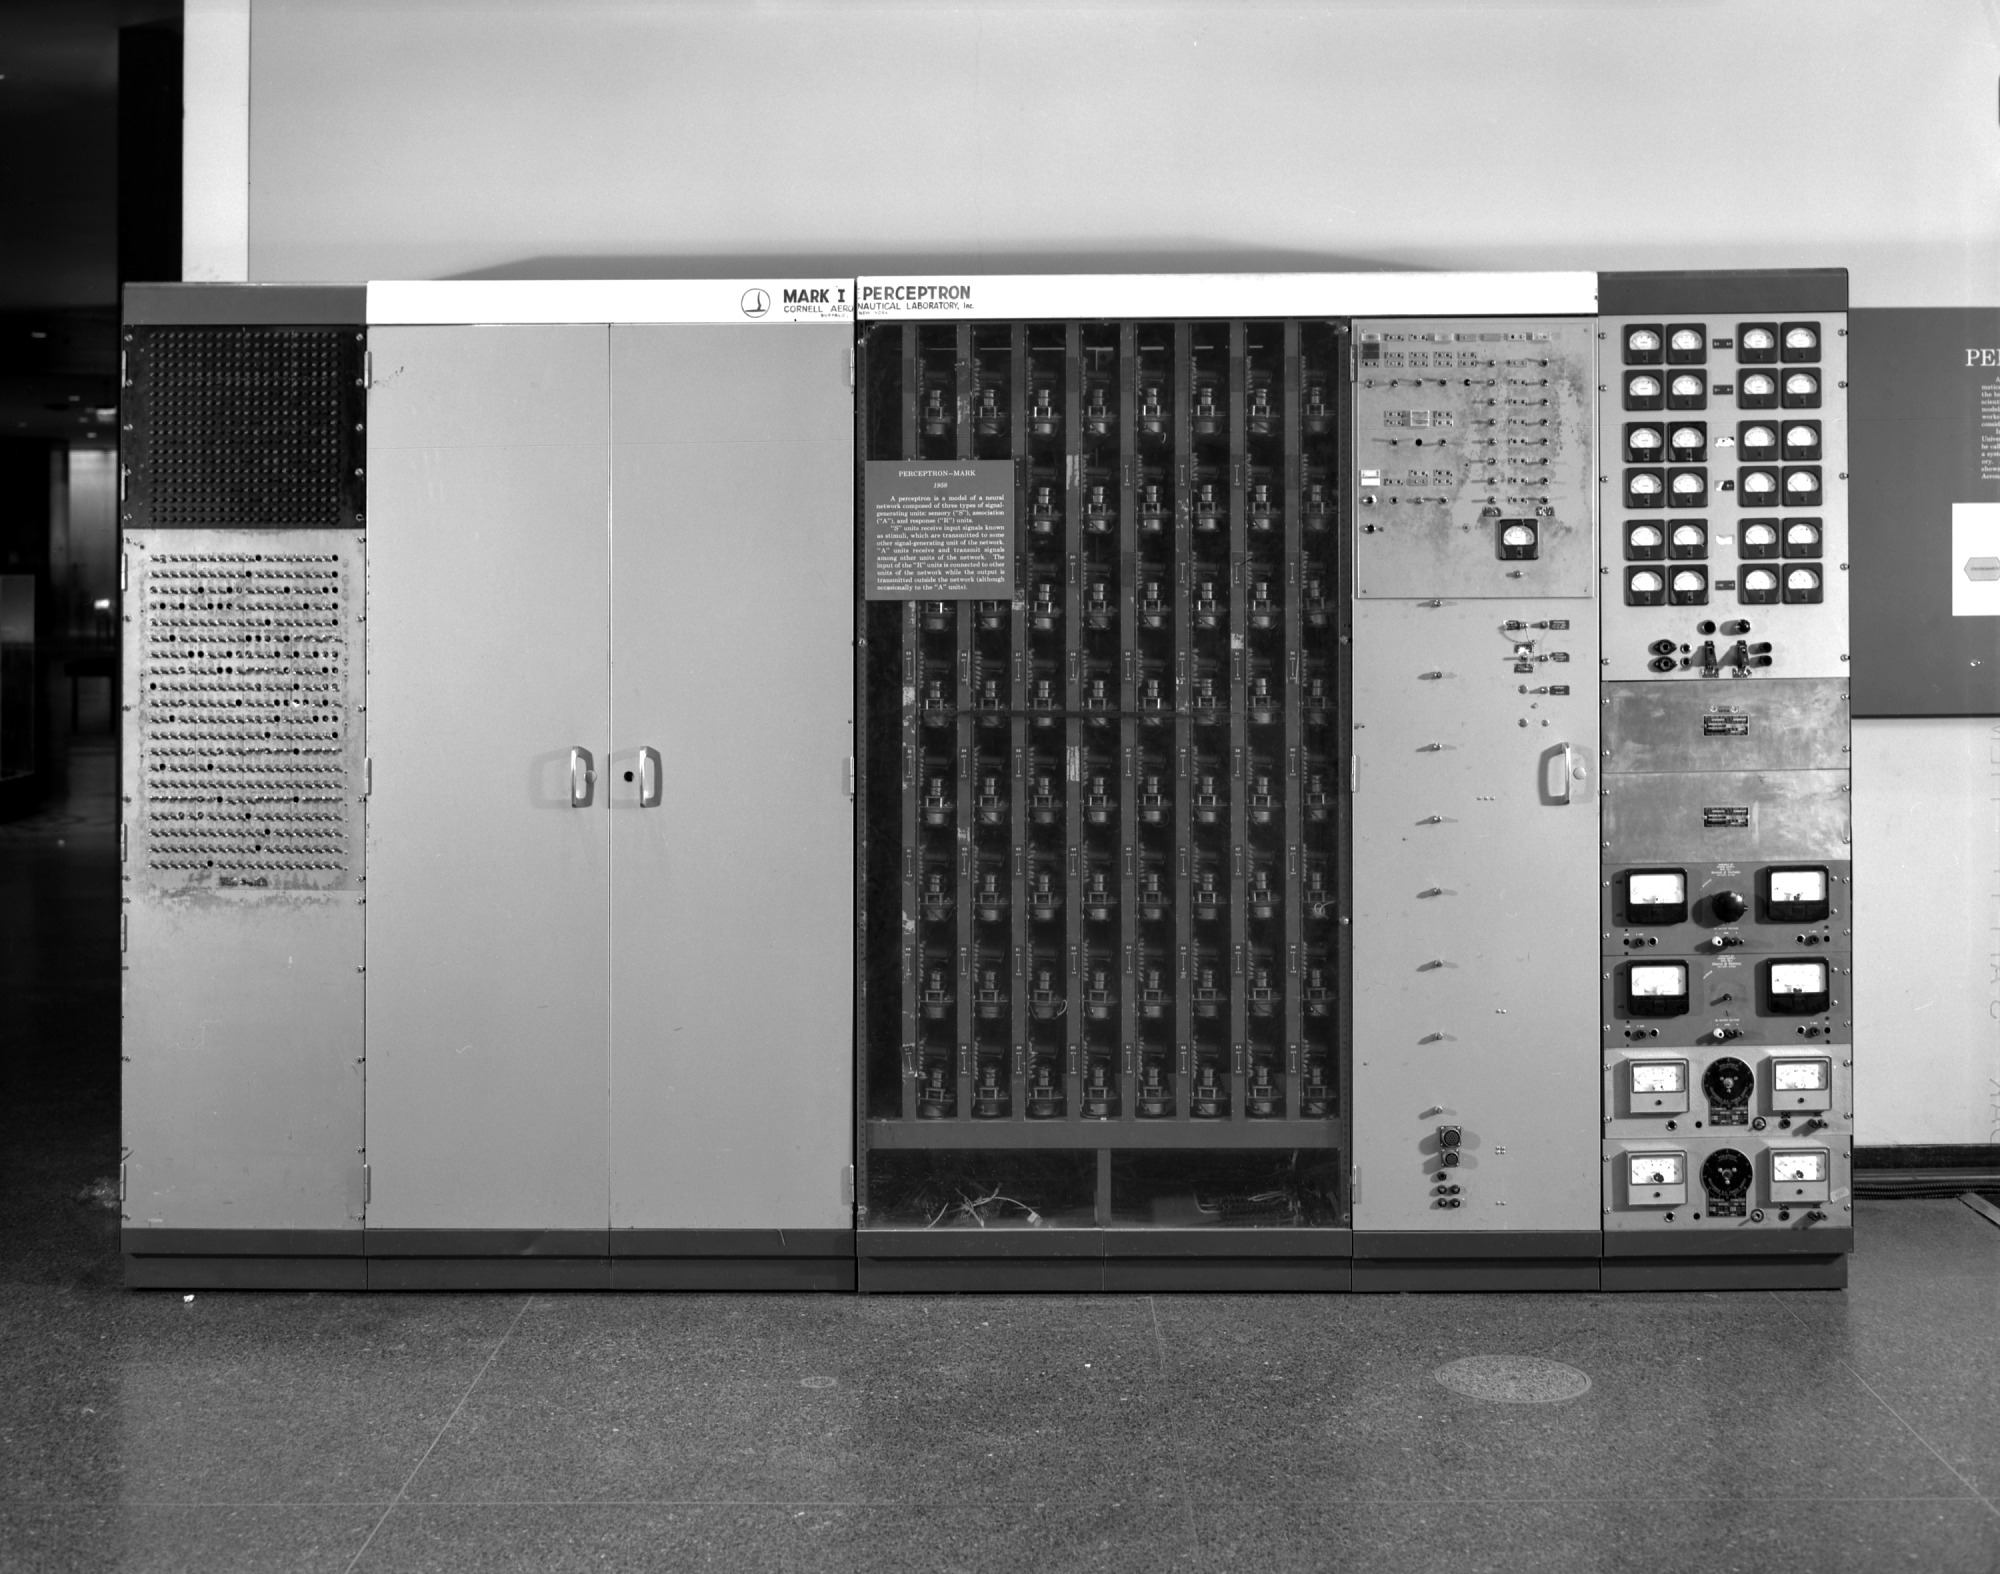
\includegraphics[height=.7\textheight]{MarkI_perceptron_2.jpg}

            \footnotesize
            A Mark I Perceptron computer - National Museum of American History
        \end{column}
    \end{columns}
\end{frame}

\begin{frame}
    {Forward propagation}
    The calculations performed by a ANN are very simple.

    \centering
    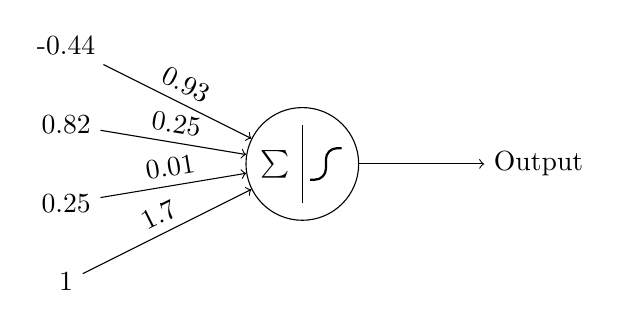
\begin{tikzpicture}
        % Neuron
        \node [draw, fill=white, circle, minimum height=4em] (n) at(3, 1.5) {$\sum\qquad$};

        % Bias
        \node (b) at(0, 0) {1};
        \draw [->] (b) -- node [above, midway, sloped] {1.7} (n);

        % Inputs and weights

        \node (i1) at (0, 1) {0.25};
        \node (i2) at (0, 2) {0.82};
        \node (i3) at (0, 3) {-0.44};

        \draw [->] (i1) -- node [above, midway, sloped] {0.01} (n);
        \draw [->] (i2) -- node [above, midway, sloped] {0.25} (n);
        \draw [->] (i3) -- node [above, midway, sloped] {0.93} (n);

        \node (out) at(6, 1.5) {Output};
        \draw [->] (n) -- (out);

        \draw [thick, rounded corners] (3.1, 1.3) -- (3.3, 1.3) -- (3.3, 1.7) -- (3.5, 1.7);

        \draw (3, 1) -- (3, 2);
    \end{tikzpicture}

    We calculate:
    \Large
    $\sum_i(x_i\cdot w_i) + b = 0.25 * 0.01 + 0.82 * 0.25 - 0.44 * 0.93 + 1.7 = \mathbf{1.498}$ and we pass it through the activation function.

    For example, using the sigmoid we get $\frac{1}{1 + e^{-1.498}} = \mathbf{0.9}$.
\end{frame}

\begin{frame}
    {Multi-layer perceptrons}
    We can extend the perceptron to a \textbf{multi-layer perceptron} (MLP).

    \centering
    % From https://github.com/davidstutz/latex-resources/blob/master/tikz-multilayer-perceptron/multilayer-perceptron.tex
    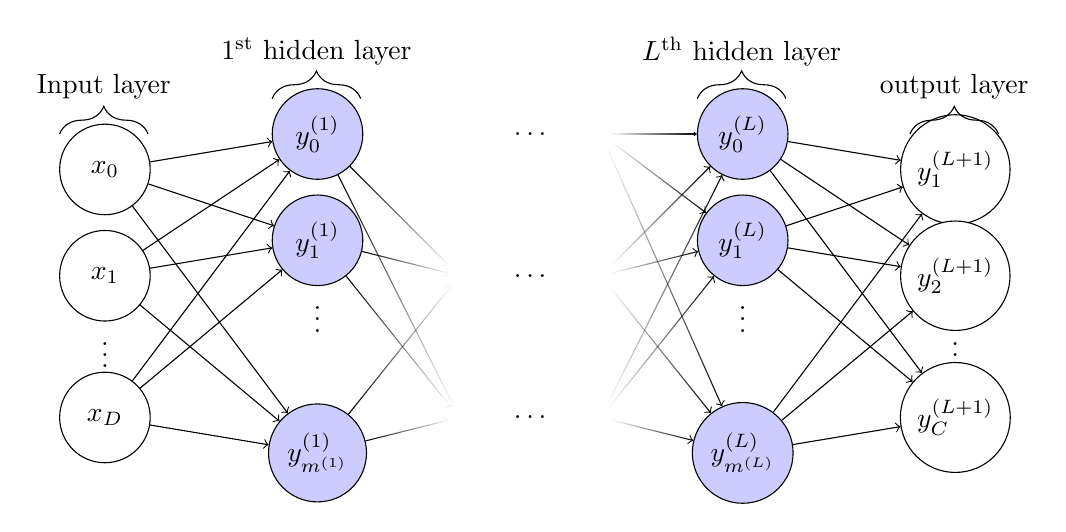
\begin{tikzpicture}[scale=0.9]
        \tikzstyle{unit}=[draw,fill=white,shape=circle,minimum size=1.15cm]
        %\tikzstyle{hidden}=[draw,shape=circle,fill=black!25,minimum size=1.15cm]
        \tikzstyle{hidden}=[draw,fill=blue!20!white,shape=circle,minimum size=1.15cm]

        \node[unit](x0) at (0,3.5){$x_0$};
        \node[unit](x1) at (0,2){$x_1$};
        \node at (0,1){\vdots};
        \node[unit](xd) at (0,0){$x_D$};

        \node[hidden](h10) at (3,4){$y_0^{(1)}$};
        \node[hidden](h11) at (3,2.5){$y_1^{(1)}$};
        \node at (3,1.5){\vdots};
        \node[hidden](h1m) at (3,-0.5){$y_{m^{(1)}}^{(1)}$};

        \node(h22) at (5,0){};
        \node(h21) at (5,2){};
        \node(h20) at (5,4){};

        \node(d3) at (6,0){$\ldots$};
        \node(d2) at (6,2){$\ldots$};
        \node(d1) at (6,4){$\ldots$};

        \node(hL12) at (7,0){};
        \node(hL11) at (7,2){};
        \node(hL10) at (7,4){};

        \node[hidden](hL0) at (9,4){$y_0^{(L)}$};
        \node[hidden](hL1) at (9,2.5){$y_1^{(L)}$};
        \node at (9,1.5){\vdots};
        \node[hidden](hLm) at (9,-0.5){$y_{m^{(L)}}^{(L)}$};

        \node[unit](y1) at (12,3.5){$y_1^{(L+1)}$};
        \node[unit](y2) at (12,2){$y_2^{(L+1)}$};
        \node at (12,1){\vdots};
        \node[unit](yc) at (12,0){$y_C^{(L+1)}$};

        \draw[->] (x0) -- (h10);       
        \draw[->] (x0) -- (h11);
        \draw[->] (x0) -- (h1m);

        \draw[->] (x1) -- (h10);
        \draw[->] (x1) -- (h11);
        \draw[->] (x1) -- (h1m);

        \draw[->] (xd) -- (h10);
        \draw[->] (xd) -- (h11);
        \draw[->] (xd) -- (h1m);

        \draw[->] (hL0) -- (y1);
        \draw[->] (hL0) -- (yc);
        \draw[->] (hL0) -- (y2);

        \draw[->] (hL1) -- (y1);
        \draw[->] (hL1) -- (yc);
        \draw[->] (hL1) -- (y2);

        \draw[->] (hLm) -- (y1);
        \draw[->] (hLm) -- (y2);
        \draw[->] (hLm) -- (yc);

        \draw[->,path fading=east] (h10) -- (h21);
        \draw[->,path fading=east] (h10) -- (h22);

        \draw[->,path fading=east] (h11) -- (h21);
        \draw[->,path fading=east] (h11) -- (h22);

        \draw[->,path fading=east] (h1m) -- (h21);
        \draw[->,path fading=east] (h1m) -- (h22);

        \draw[->,path fading=west] (hL10) -- (hL0);
        \draw[->,path fading=west] (hL12) -- (hL0);
        \draw[->,path fading=west] (hL11) -- (hL0);

        \draw[->,path fading=west] (hL10) -- (hL1);
        \draw[->,path fading=west] (hL11) -- (hL1);
        \draw[->,path fading=west] (hL12) -- (hL1);

        \draw[->,path fading=west] (hL10) -- (hLm);
        \draw[->,path fading=west] (hL11) -- (hLm);
        \draw[->,path fading=west] (hL12) -- (hLm);

        \draw [decorate,decoration={brace,amplitude=10pt},xshift=-4pt,yshift=0pt] (-0.5,4) -- (0.75,4) node [black,midway,yshift=+0.6cm]{Input layer};
        \draw [decorate,decoration={brace,amplitude=10pt},xshift=-4pt,yshift=0pt] (2.5,4.5) -- (3.75,4.5) node [black,midway,yshift=+0.6cm]{$1^{\text{st}}$ hidden layer};
        \draw [decorate,decoration={brace,amplitude=10pt},xshift=-4pt,yshift=0pt] (8.5,4.5) -- (9.75,4.5) node [black,midway,yshift=+0.6cm]{$L^{\text{th}}$ hidden layer};
        \draw [decorate,decoration={brace,amplitude=10pt},xshift=-4pt,yshift=0pt] (11.5,4) -- (12.75,4) node [black,midway,yshift=+0.6cm]{output layer};
    \end{tikzpicture}

    \pause
    MLPs have one or more \textbf{hidden layers} that are connected to the input layer. By increasing the complexity of the network, it can perform much more complex tasks.

    This is called the \textbf{universal approximation theorem}.
\end{frame}

\begin{frame}
    {Forward propagation in an MLP}
    Forward propagation in an MLP is similar to what we just saw for a single neuron.

    \pause

    \begin{itemize}[<+->]
        \item We start from the first hidden layer
        \item We calculate the output of each neuron as the weighted sum of the inputs plus the bias, then pass it through the activation function.
        \item The output of this hidden layer is used as input for the next hidden layer.
        \item We repeat this process until we reach the output layer.
    \end{itemize}

\end{frame}
\begin{frame}
    {Activation function}
    Several activation functions are used in ANNs. They are used to introduce non-linearity in the ANN.

    Some of the most common are:
    \begin{columns}
        \begin{column}{.5\textwidth}
            \begin{itemize}
                \item Sigmoid
                \item Hyperbolic tangent (tanh)
                \item Rectified linear unit (ReLU)
                \item Leaky ReLU
            \end{itemize}
        \end{column}
        \begin{column}{.5\textwidth}
            $$\sigma(x) = \frac{1}{1 + e^{-x}}$$
            $$\tanh(x) = \frac{e^{x} - e^{-x}}{e^{x} + e^{-x}}$$
            $$\text{ReLU}(x) = \max(0, x)$$
            $$\text{ReLU}(x, a) = \max(a\cdot x, x)$$
        \end{column}
    \end{columns}
    \centering
    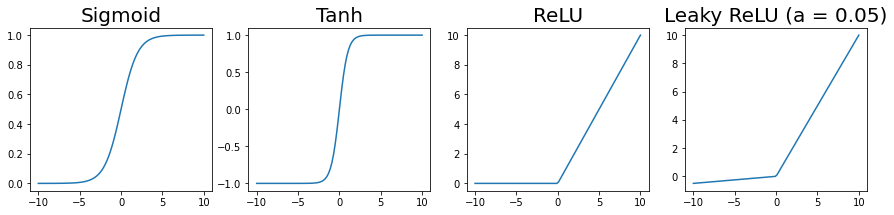
\includegraphics[width=\textwidth]{activation.png}
\end{frame}

\section{Optimization (how does the ANN learn?)}

\begin{frame}
    {Backpropagation}
    Once the forward propagation is complete, we can start \textbf{backpropagation}.

    This is the process of improving the weights of each node to minimise the error in the output of the network.

    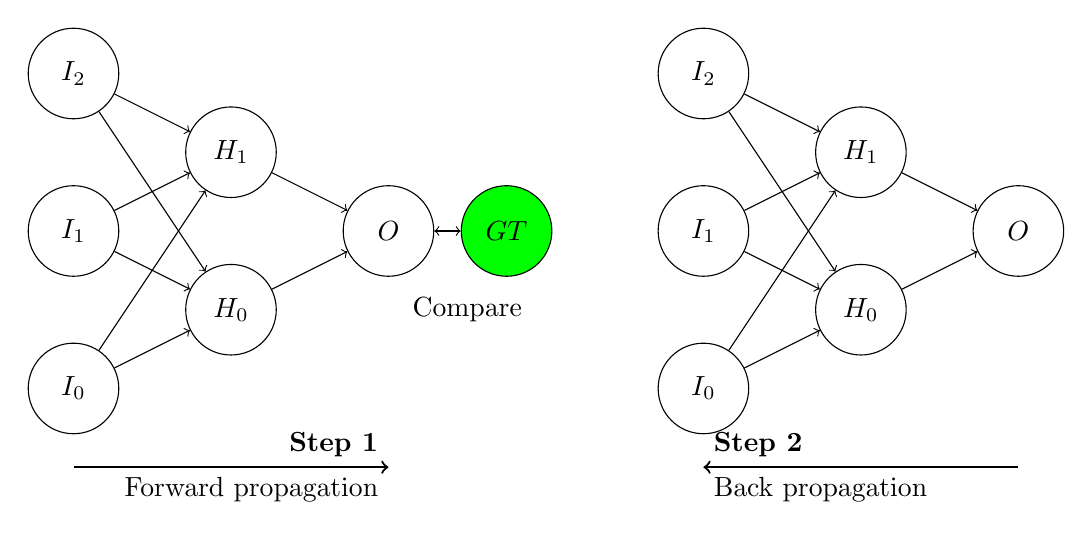
\begin{tikzpicture}
        \tikzstyle{unit}=[draw,fill=white,shape=circle,minimum size=1.15cm]

        \node[unit](x0) at (0,0){$I_0$};
        \node[unit](x1) at (0,2){$I_1$};
        \node[unit](x2) at (0,4){$I_2$};

        \node[unit](h0) at (2,1){$H_0$};
        \node[unit](h1) at (2,3){$H_1$};

        \node[unit](y0) at (4,2){$O$};

        \draw[->] (x0) -- (h0);
        \draw[->] (x1) -- (h0);
        \draw[->] (x2) -- (h0);
        \draw[->] (x0) -- (h1);
        \draw[->] (x1) -- (h1);
        \draw[->] (x2) -- (h1);
        \draw[->] (h0) -- (y0);
        \draw[->] (h1) -- (y0);

        \draw[thick, ->] (0, -1) -- (4, -1) node [below, anchor=north east]{Forward propagation} node [above, anchor=south east]{\textbf{Step 1}};

        \pause
        \only <2>{
            \node[unit, fill = green](GT) at (5.5,2){$GT$};
            \draw [<->] (y0) -- (GT);
            \node at (5, 1) {Compare};
        }
        \pause

        \node[unit](x0) at (8,0){$I_0$};
        \node[unit](x1) at (8,2){$I_1$};
        \node[unit](x2) at (8,4){$I_2$};

        \node[unit](h0) at (10,1){$H_0$};
        \node[unit](h1) at (10,3){$H_1$};

        \node[unit](y0) at (12,2){$O$};

        \draw[->] (x0) -- (h0);
        \draw[->] (x1) -- (h0);
        \draw[->] (x2) -- (h0);
        \draw[->] (x0) -- (h1);
        \draw[->] (x1) -- (h1);
        \draw[->] (x2) -- (h1);
        \draw[->] (h0) -- (y0);
        \draw[->] (h1) -- (y0);

        \draw[thick, ->] (12, -1) -- (8, -1) node [below, anchor=north west]{Back propagation} node [above, anchor=south west]{\textbf{Step 2}};

    \end{tikzpicture}
\end{frame}

\begin{frame}
    {The training process}
    During training:

    \begin{itemize}[<+->]
        \item We initialize the weights of the network with random numbers.
        \item We pass data and ground truth through the ANN and do a forward pass.
        \item We calculate the error in the output layer. This is done with a \textbf{loss function} (or \textbf{cost function}).
        \item We now use an \textbf{optimizer} to update the weights to minimise the loss.
        \item We run a forward pass again and repeat the process until the loss is small enough or we reach a maximum number of iterations.
    \end{itemize}

    \pause
    One of the most common optimizers is \textbf{gradient descent} (or some of its variations).
\end{frame}

\begin{frame}
    {Gradient descent}
    \begin{itemize}[<+->]
        \item \textbf{Gradient descent} works by calculating how much the loss changes depending on each weight.
        \item It does so by calculating the partial derivative of the loss with respect to each weight (the gradient!)
        \item It then takes a step in the direction of the gradient to go towards the minimum of the loss.
        \item The bigger the loss, the bigger the step it takes.
        \item We control this using a parameter called \textbf{learning rate} ($\alpha$).
    \end{itemize}
    \pause
    \begin{columns}
        \begin{column}{.5\textwidth}
            \centering
            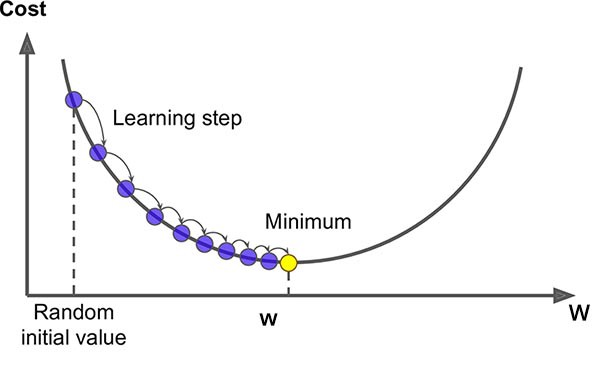
\includegraphics[width=\textwidth]{gradient_descent.jpg}
        \end{column}
        \begin{column}{.5\textwidth}
            \LARGE
            $\mathbf{w} \leftarrow \mathbf{w} - \alpha \nabla J(\mathbf{w})$

            \vspace{2em}
            \footnotesize
            $\leftarrow$ While the image shows a single weight, in reality we need to do this for the (very) large number of parameters in the network!
        \end{column}
    \end{columns}
\end{frame}

\begin{frame}
    {Learning rate}
    The choice of learning rate is key!
    \centering
    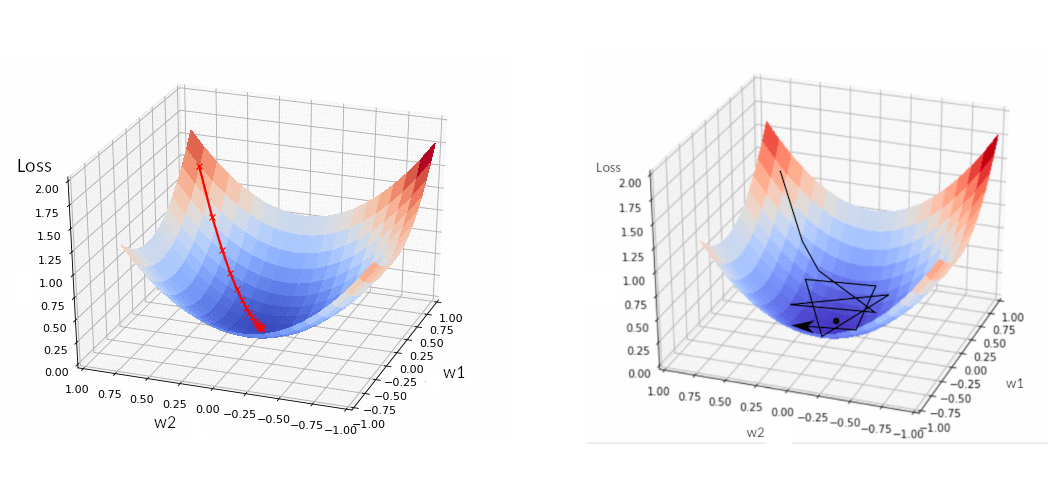
\includegraphics[width=\textwidth]{learningrate.jpg}
\end{frame}

\begin{frame}
{Next lecture...}
Having a general understanding of ANNs, we will look at more complex networks and start talking about deep learning!
\end{frame}
\end{document}